\documentclass[11pt,a4paper]{article}

\usepackage[margin=1in]{geometry}
\usepackage{amsmath,amssymb,amsthm}
\usepackage{booktabs}
\usepackage{graphicx}
\usepackage{hyperref}
\usepackage{natbib}
\usepackage{xcolor}
\usepackage{microtype}
\usepackage{setspace}
\usepackage{caption}
\usepackage{subcaption}

\hypersetup{
  colorlinks=true,
  linkcolor=blue!50!black,
  citecolor=blue!50!black,
  urlcolor=blue!60!black
}

\newtheorem{definition}{Definition}
\newtheorem{remark}{Remark}

\title{Fisher Geometry of a Live Decision-Model API:\\
Ticket Triage Sensitivity under TypeSafe}
\author{
  Heath Li\\
  \texttt{Kunyanli230/Jevometry}\\
  \small Working draft toward JAAMAS / arXiv
}
\date{\today}

\begin{document}
\maketitle

\begin{abstract}
Decision-model APIs expose calibrated categorical distributions over
operational questions---request type, escalation need, impact---conditioned on
structured ticket state. Practitioners routinely treat those distributions as
point predictions; less often do they ask how \emph{sensitive} the reported law
is to the continuous parameters that define the ticket (dollar amount, wait
time). This paper studies that sensitivity for a live TypeSafe decision model
using the Jevometry geometry stack: finite-difference Jacobians, Fisher
information on each node, entropy, and an explicit capability matrix that
refuses unsupported claims.

We first show that an aggressive finite-difference stencil
($h_{\mathrm{amount}}{=}1.0$, $h_{\mathrm{wait}}{=}0.25$ with a two-scale
stability check) marks all three live node geometries
\texttt{unstable}/\texttt{step\_stability\_exceeded}, so Fisher traces cannot
be trusted. Shrinking steps to $0.25$ and $0.05$ and using a single-scale live
stencil restores \texttt{ok} Jacobian and Fisher status on every node while
preserving the qualitative finding that wait-time diagonals dominate amount.
A fresh live re-run (75 traces, zero failures) yields centre-point entropies
$H\!\approx\!1.04/0.50/0.31$~nats for
\texttt{request\_type}/\texttt{needs\_escalation}/\texttt{impact}, with Fisher
traces $\mathrm{tr}(I)\!\approx\!0.86/0.085/2.61$. Two nodes remain
rank-deficient (\texttt{not\_identifiable}), and system/action Fisher stay
\texttt{unsupported} because no joint model is declared and routing is
deterministic. An offline analytic twin on a $3{\times}3$ grid provides a
noise-free contrast. Together, the study is a template for honest geometry of
commercial decision APIs: report entropy when Fisher is unstable, shrink
stencils before claiming sensitivity, and separate node geometry from joint or
policy claims. Code, CSV summaries, and figures ship with Jevometry
(\texttt{papers/typesafe-ticket/}).
\end{abstract}

\section{Introduction}

Ticket triage is a canonical multi-question decision workflow. Given a
structured ticket---amount in USD, hours already waiting, channel, free-text
summary---a decision model returns categorical distributions over (i)~request
type (billing / technical / refund), (ii)~whether escalation is needed, and
(iii)~impact severity. Production systems then map those answers into a
deterministic routing label (standard queue, priority, refund review,
escalate). Large language models and specialized decision APIs have made such
distributions cheap to obtain~\citep{yao2023react,park2023generative,typesafe2026},
but cheap does not mean geometrically well-behaved: finite-difference
estimates of $\partial_\theta P$ can fail stability checks under API noise,
and without a declared joint the three marginals do not determine a system
Fisher matrix~\citep{jevometry2026}.

Information-theoretic multi-agent sensing and Dec-POMDP active perception
optimize mutual information, prediction rewards, or belief-dependent
payoffs~\citep{lauri2020prediction,lauri2020decpomdp,oliehoek2016decpomdp,shi2026imas2,molloy2023smoother,corah2021scalable}.
Those lines choose \emph{what to observe}. A companion paper studies
\emph{which coordination rule} retains Fisher information after action
aggregation~\citep{li2026coordfisher}. Here the complementary question is
narrower and more operational: \emph{given a fixed live decision model and a
fixed question set, how sensitive are the reported node distributions to
ticket parameters, and when is that sensitivity trustworthy?}

\paragraph{Contributions.}
\begin{enumerate}
  \item We document a live TypeSafe ticket experiment in Jevometry, including
  the capability matrix that correctly marks system/action Fisher and
  likelihood-based inference as unsupported.
  \item We show that stencil choice is first-order: the original live steps
  yield \texttt{step\_stability\_exceeded} on all nodes; shrinking amount and
  wait steps and switching live to a single-scale stencil restores
  \texttt{ok} node geometry.
  \item We report reproducible centre-point entropy and Fisher summaries from a
  fresh live re-run, with wait-hours diagonals dominating amount, plus an
  offline synthetic grid for noise-free comparison.
  \item We state limitations honestly: rank deficiency on binary/score nodes,
  no joint model, deterministic policy, and API non-determinism across
  re-runs.
\end{enumerate}

\section{Related work}

\paragraph{Active perception and Dec-POMDPs.}
Prediction-reward formulations~\citep{lauri2020prediction} and
policy-graph improvements for information gathering~\citep{lauri2020decpomdp}
optimize belief-dependent objectives under decentralization. Classical POMDP
planning emphasizes value of information under partial
observability~\citep{kaelbling1998planning,oliehoek2016decpomdp}. IMAS$^2$
adds joint agent selection under mutual-information
objectives~\citep{shi2026imas2}. Our setting does not choose sensors; it
\emph{audits} a deployed question set.

\paragraph{Fisher geometry and DPI.}
Fisher information is the local Riemannian metric of a parametric
family~\citep{fisher1925theory,amari2016information,amari1998natural}.
Data-processing inequalities constrain pushforwards~\citep{zamir1998fisherdpi,cover2006elements}.
Sensor placement and mutual-information maximization provide algorithmic
templates~\citep{krause2008near} but assume controllable observation design.

\paragraph{LLM / agent decision stacks.}
Tool-using and multi-agent LLM systems~\citep{yao2023react,park2023generative}
expose decision surfaces that look like categorical models. Geometry on those
surfaces is rarely reported. TypeSafe is treated here as a black-box
decision-model API accessed through an official Python
SDK~\citep{typesafe2026}; we do not reverse-engineer model internals.

\paragraph{Companion coordination paper.}
\citet{li2026coordfisher} hold analytic agent laws fixed and vary
deterministic aggregation maps, ranking rules by Fisher loss after the action
layer. The present paper holds the live API fixed and studies parameter
sensitivity of the reported node laws---orthogonal axes of the same Jevometry
programme~\citep{jevometry2026}.

\section{Method}

\subsection{Ticket decision model}

Let $\theta=(\mathrm{amount},\mathrm{wait\_hours})\in\mathbb{R}^2$ with
design centre $\theta_\star=(250,8)$ (USD, hours). The live adapter renders a
structured state and queries three TypeSafe questions:
\begin{itemize}
  \item \texttt{request\_type}: Choice on $\{\mathrm{billing},\mathrm{technical},\mathrm{refund}\}$;
  \item \texttt{needs\_escalation}: Noul (binary) on $\{\mathrm{false},\mathrm{true}\}$;
  \item \texttt{impact}: Score on $\{0,1,2\}$ (low/medium/high).
\end{itemize}
Routing semantics are declared \texttt{deterministic\_policy}: the production
map from reported probabilities to an action label is not a sampling model, so
trajectory/action Fisher are refused by the capability matrix.

\subsection{Node Fisher via finite differences}

For a node with reported probabilities $P_\theta\in\Delta^{K-1}$, Jevometry
estimates a Jacobian $J\approx\partial_\theta P$ by centered finite differences
along each parameter, optionally at multiple step scales, then forms
\begin{equation}
  I(\theta)=J^\top \mathrm{diag}(P_\theta)^{-1} J
\end{equation}
when regularity checks pass~\citep{jevometry2026}. Entropy
$H(P)=-\sum_k P_k\log P_k$ is always available from the reported distribution
and does not require a stable Jacobian.

\begin{definition}[Relative step stability]
A multi-scale stencil compares Jacobians at step $h$ and $h/2$. If the
relative discrepancy exceeds a threshold (default $0.10$), the geometry is
marked \texttt{unstable} with reason \texttt{step\_stability\_exceeded}.
Unstable Fisher values may still be printed as diagnostics but are not
validated geometry.
\end{definition}

\subsection{Stencil shrink for live APIs}

Live API responses are noisy across repeats. Empirically, the original live
defaults $h_{\mathrm{amount}}{=}1.0$, $h_{\mathrm{wait}}{=}0.25$ with
\texttt{step\_scales}$=[1.0,0.5]$ failed the multi-scale check on every node.
We adopt:
\begin{itemize}
  \item $h_{\mathrm{amount}}{=}0.25$, $h_{\mathrm{wait}}{=}0.05$;
  \item live stencil \texttt{step\_scales}$=[1.0]$ (single scale);
  \item offline synthetic keeps the two-scale stability stencil.
\end{itemize}
Repeats remain $5$ with a live budget cap of $100$ attempts; the acquisition
plan expects $25$ requests at the single centre point used for live.

\subsection{Offline synthetic twin}

The analytic \texttt{TicketSystemAdapter} defines softmax logits that depend
smoothly on scaled amount and wait~\citep{jevometry2026}. Offline runs a
$3{\times}3$ grid
$\mathrm{amount}\in\{100,250,600\}$,
$\mathrm{wait\_hours}\in\{2,8,30\}$
and reports node geometry plus a declared product \emph{surrogate} action
distribution (explicitly not the production routing law).

\subsection{What we refuse to claim}

Without a declared joint $P_\theta(Z_1,Z_2,Z_3)$, system Fisher is
\texttt{unsupported}/\texttt{no\_joint\_model}. With deterministic routing,
action Fisher is \texttt{unsupported}/\texttt{deterministic\_policy}. Without
a sampling contract, CRLB-style inference is refused. These refusals are
features of the analysis object model, not bugs.

\section{Experiments}

\subsection{Protocol}

All commands from the repository root:
\begin{verbatim}
uv sync --locked
uv run python examples/jev_ticket_sensitivity/run.py
# optional:
uv run python examples/jev_ticket_sensitivity/run.py --live
uv run python examples/jev_ticket_sensitivity/paper_export.py
\end{verbatim}
Credentials: environment variables \texttt{TYPESAFE\_API\_KEY} and
\texttt{TYPESAFE\_MODEL} (values never committed). Live outputs under
\texttt{examples/jev\_ticket\_sensitivity/output/} are gitignored; paper tables
are summarized into \texttt{papers/typesafe-ticket/data/}.

\subsection{Before vs after stencil shrink}

\begin{figure}[t]
\centering
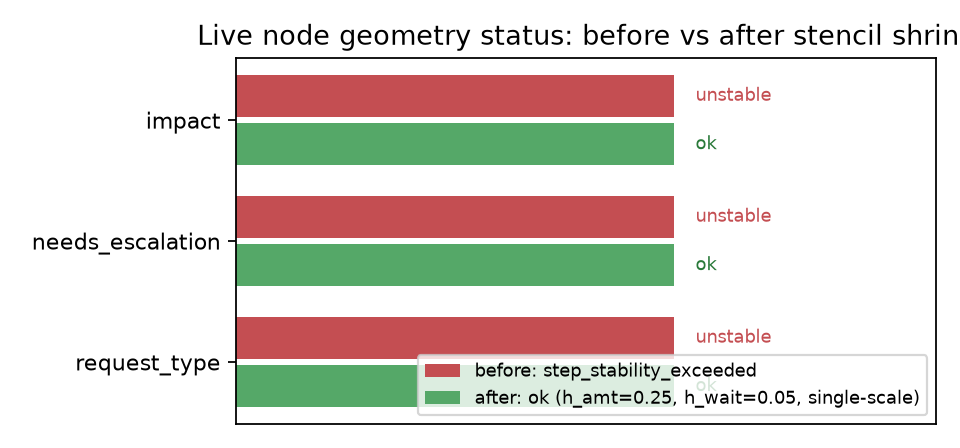
\includegraphics[width=0.85\linewidth]{figures/stability_before_after.png}
\caption{Live node geometry status before and after the stencil shrink
(PR~\texttt{fix/ticket-live-stencil-stability}). Before: all three nodes
\texttt{unstable}/\texttt{step\_stability\_exceeded}. After: all
\texttt{ok}.}
\label{fig:stability}
\end{figure}

Figure~\ref{fig:stability} summarizes the status flip. We deliberately do
\emph{not} treat pre-fix Fisher numbers as validated results.

\subsection{Live centre-point results (fresh re-run)}

A live re-run after the stencil fix completed with $75$ traces, $0$ failures,
\texttt{incomplete=False}, run id
\texttt{ticket-sensitivity-live-20261010T143812-0}
(UTC timestamp in \texttt{summary.json}).

\begin{table}[t]
\centering
\caption{Live TypeSafe centre point $\theta_\star=(250,8)$ after stencil
shrink. Fisher status is \texttt{ok} on all nodes; identifiability remains
rank-deficient for escalation and impact.}
\label{tab:live}
\begin{tabular}{lrrrrr}
\toprule
Node & $H$ (nats) & $\mathrm{tr}(I)$ & $I_{\mathrm{amt}}$ & $I_{\mathrm{wait}}$ & Ident.\\
\midrule
request\_type & $1.040$ & $0.858$ & $0.138$ & $0.720$ & --- \\
needs\_escalation & $0.500$ & $0.085$ & $0.0225$ & $0.0625$ & rank-def.\\
impact & $0.309$ & $2.613$ & $0.154$ & $2.460$ & rank-def.\\
\bottomrule
\end{tabular}
\end{table}

\begin{figure}[t]
\centering
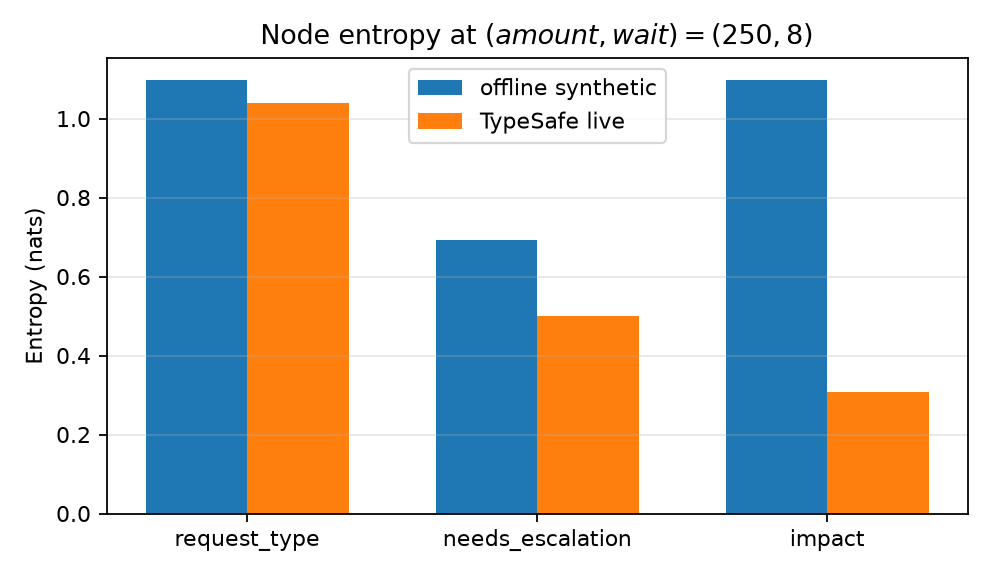
\includegraphics[width=0.85\linewidth]{figures/entropy_center.png}
\caption{Entropy at the design centre: offline synthetic vs TypeSafe live.}
\label{fig:entropy}
\end{figure}

\begin{figure}[t]
\centering
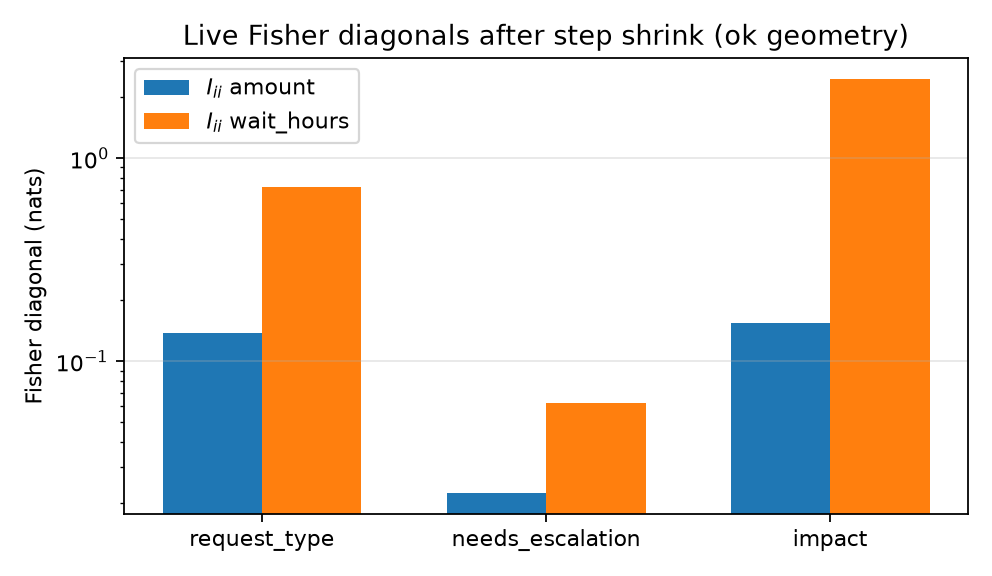
\includegraphics[width=0.85\linewidth]{figures/fisher_diag_live.png}
\caption{Live Fisher diagonals (log scale). Wait-hours dominates amount on
every node after the stencil shrink.}
\label{fig:fisher}
\end{figure}

Table~\ref{tab:live} and Figures~\ref{fig:entropy}--\ref{fig:fisher} show:
(i)~entropy is highest for \texttt{request\_type} and lowest for
\texttt{impact}; (ii)~$\mathrm{tr}(I)$ is dominated by the wait-hours
diagonal; (iii)~binary/score nodes can be Fisher-ok yet
\texttt{not\_identifiable} (rank-deficient $I$), so local invertibility fails
even when stability passes.

\subsection{Capability matrix}

\begin{table}[t]
\centering
\caption{Capability matrix (identical structure for live and offline).}
\label{tab:caps}
\begin{tabular}{lll}
\toprule
Capability & Status & Reason \\
\midrule
distribution\_comparison & ok & --- \\
node\_geometry & ok & --- \\
system\_information & unsupported & no\_joint\_model \\
action\_information & unsupported & deterministic\_policy \\
inference & unsupported & no\_likelihood\_model \\
\bottomrule
\end{tabular}
\end{table}

\subsection{Offline synthetic grid}

\begin{figure}[t]
\centering
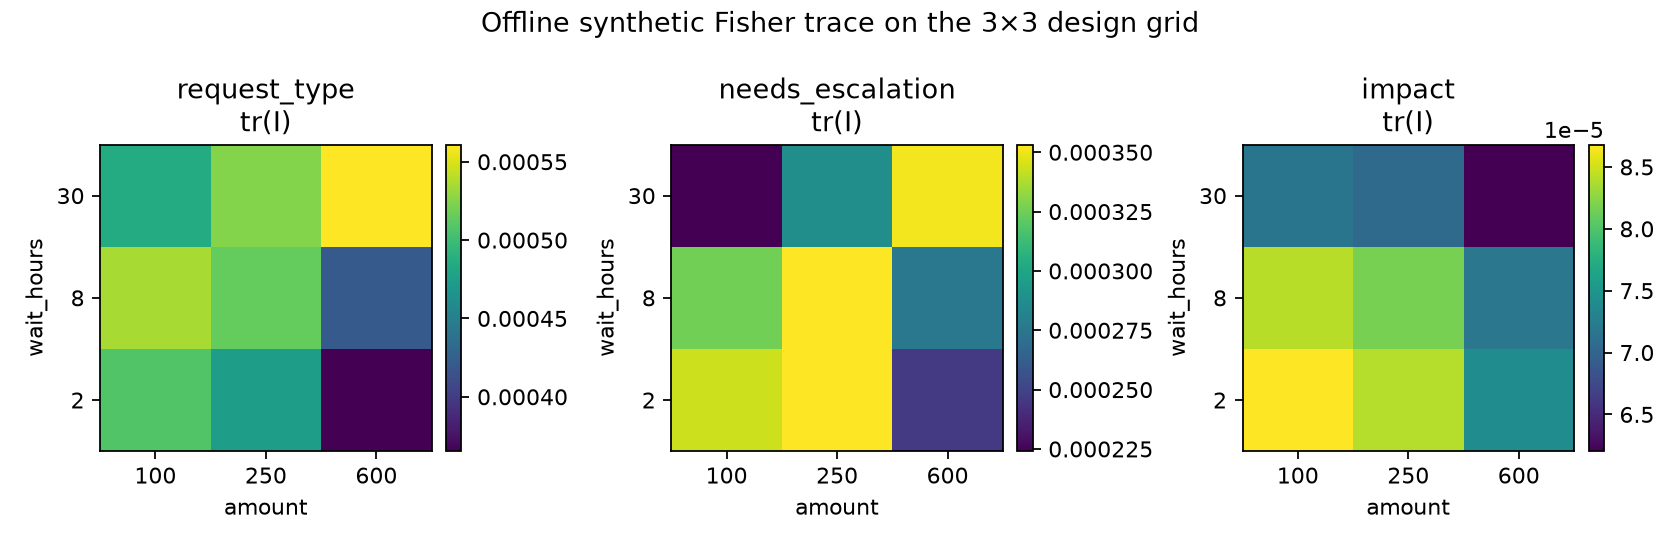
\includegraphics[width=\linewidth]{figures/synth_fisher_grid.png}
\caption{Offline synthetic $\mathrm{tr}(I)$ on the $3{\times}3$ design grid.
Traces are small relative to live (analytic logits change slowly in raw
parameter units) but remain \texttt{ok} under the two-scale stencil.}
\label{fig:grid}
\end{figure}

At the shared centre, synthetic entropies are
$H\!\approx\!1.097/0.692/1.098$ with tiny Fisher traces
($\mathrm{tr}(I)\!\sim\!10^{-4}$--$10^{-5}$). The live model is a different
law: absolute Fisher scales are not comparable across providers, but the
\emph{status} and \emph{relative} wait$>$amount pattern are.

\section{Discussion}

\paragraph{Stencil first, narrative second.}
Publishing Fisher numbers from an unstable stencil would overstate
sensitivity. The capability/status channel is the right gate: entropy remains
reportable; Fisher waits for \texttt{ok}.

\paragraph{Wait-time sensitivity.}
Across live nodes, $I_{\mathrm{wait}}\gg I_{\mathrm{amt}}$ at $\theta_\star$.
Operationally, wait-time interventions move the reported distributions more
than small amount perturbations at this centre---subject to the scale
normalization in the ParameterSpec ($100$~USD, $12$~hours).

\paragraph{Identifiability vs stability.}
Stability says the finite-difference Jacobian is repeatable at the chosen $h$.
Identifiability asks whether $I$ has full parameter rank. Binary nodes with
two-dimensional $\theta$ are structurally prone to rank deficiency; treating
\texttt{ok} Fisher as ``fully informative about both parameters'' would be
incorrect.

\paragraph{Relation to coordination loss.}
If a council later compresses these three nodes through a deterministic
aggregator, Fisher loss after the action layer can be measured as in
\citet{li2026coordfisher}---but only after a joint is declared. The live
ticket example currently stops at node geometry by design.

\section{Limitations}

\begin{itemize}
  \item \textbf{Single live centre.} Budget limits live to $\theta_\star$;
  grid conclusions use the synthetic twin.
  \item \textbf{API non-determinism.} Re-runs change numerical Fisher values;
  we commit summaries, not raw \texttt{traces.jsonl}.
  \item \textbf{No joint / no action Fisher.} Deterministic routing and absent
  joint block system-level claims.
  \item \textbf{Black-box vendor model.} We do not claim internal TypeSafe
  training details; the object of study is the reported distribution interface.
  \item \textbf{Synthetic scale mismatch.} Analytic logits are slow in raw
  $(amount,wait)$ units, so absolute $\mathrm{tr}(I)$ is not a live
  baseline---only a methodological twin.
\end{itemize}

\section{Conclusion}

Live decision-model APIs can be placed under Fisher geometry if---and
only if---finite-difference stencils are stable. For TypeSafe ticket triage in
Jevometry, shrinking amount/wait steps and using a single-scale live stencil
turns \texttt{step\_stability\_exceeded} into \texttt{ok} node geometry,
reveals wait-dominated diagonals, and still surfaces rank-deficiency and
capability refusals that keep joint and policy claims honest. Entropy remains
the fallback when geometry fails. Future work: declare a product or tree joint
for live nodes, attach a stochastic routing surrogate for action Fisher, and
extend the live grid under a larger budget.

\section*{Reproducibility}

Branch \texttt{paper/typesafe-ticket-sensitivity}; paper artifacts under
\texttt{papers/typesafe-ticket/}; experiment code under
\texttt{examples/jev\_ticket\_sensitivity/}. Offline needs no credentials;
live requires \texttt{TYPESAFE\_API\_KEY} and \texttt{TYPESAFE\_MODEL}.



\clearpage
\appendix
\section{Experiment design details}
\label{app:design}

\paragraph{Live acquisition.}
At $\theta_\star=(250,8)$ with three nodes, five repeats, and a single-scale
centered difference along two parameters, the acquisition planner expects
$25$ TypeSafe requests (budget cap $100$). The re-run reported in
Section~4 completed with $75$ stored traces (including bookkeeping rows) and
zero failures.

\paragraph{Parameter scales.}
ParameterSpec scales are $100$~USD for amount and $12$~hours for wait.
Standardized Fisher traces rescale by these units; Tables in the main text
report raw (unstandardized) diagonals unless noted.

\paragraph{Synthetic centre comparison.}
Table~\ref{tab:syncenter} lists offline synthetic metrics at the shared
centre. Absolute Fisher scales are not comparable to live; the table is a
methodological twin under the two-scale stencil.

\begin{table}[h]
\centering
\caption{Offline synthetic centre $\theta_\star=(250,8)$.}
\label{tab:syncenter}
\begin{tabular}{lrrrr}
\toprule
Node & $H$ (nats) & $\mathrm{tr}(I)$ & $I_{\mathrm{amt}}$ & $I_{\mathrm{wait}}$ \\
\midrule
request\_type & $1.097$ & $5.15{\times}10^{-4}$ & $8.20{\times}10^{-7}$ & $5.14{\times}10^{-4}$ \\
needs\_escalation & $0.692$ & $3.53{\times}10^{-4}$ & $2.55{\times}10^{-6}$ & $3.51{\times}10^{-4}$ \\
impact & $1.098$ & $8.17{\times}10^{-5}$ & $1.31{\times}10^{-6}$ & $8.04{\times}10^{-5}$ \\
\bottomrule
\end{tabular}
\end{table}

\section{Artifact checklist}
\label{app:artifacts}

\begin{itemize}
  \item \texttt{examples/jev\_ticket\_sensitivity/run.py} --- offline + live entrypoints; stencil shrink.
  \item \texttt{examples/jev\_ticket\_sensitivity/paper\_export.py} --- CSV/JSON/PNG exporter.
  \item \texttt{papers/typesafe-ticket/data/*.csv} --- committed summaries (no API keys, no full traces).
  \item \texttt{papers/typesafe-ticket/figures/*} --- entropy, Fisher diagonals, synthetic grid, stability status.
  \item Capability refusals for system/action Fisher are intentional analysis-object boundaries.
\end{itemize}


\bibliographystyle{plainnat}
\bibliography{references}

\end{document}
